%%%%%%%%%%%%%%%%%%%%%%%%%%%%%%%%%%%%%%%%%%%%%%%%%%%%%%%%%%%%%%%%%%%%%%%%%%%%%%%%
\section{Preferences, the Filesystem, the Options Menu, and Intents}
%%%%%%%%%%%%%%%%%%%%%%%%%%%%%%%%%%%%%%%%%%%%%%%%%%%%%%%%%%%%%%%%%%%%%%%%%%%%%%%%
\subsection{Preferences}
\begin{frame}
\frametitle{Preferences}
\begin{columns}
\column{0.70\textwidth}
Preferences are user-specific settings for an application. To create preferences for our application, we need to:
\begin{enumerate}
\item Create a Preference resource file called \texttt{prefs.xml}
\item Implement the \texttt{PrefsActivity.java} file that inflates that resource file
\item Register this new activity with the \texttt{AndroidManifest.xml} file
\item Provide a way to start that activity from the rest of the application
\end{enumerate}
\column{0.25 \textwidth}
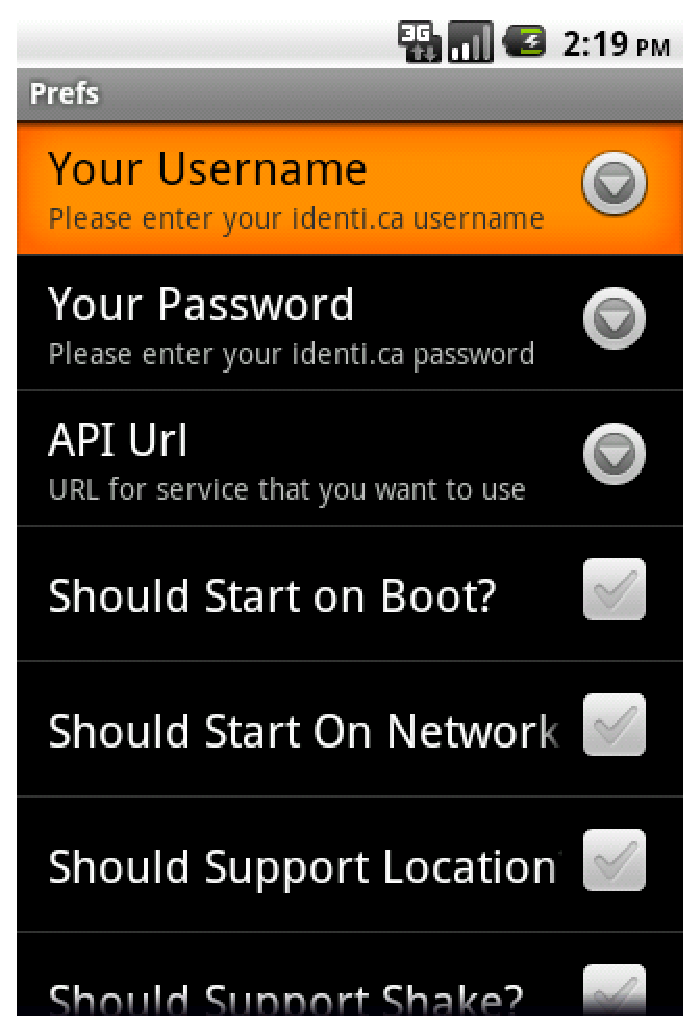
\includegraphics[width= 0.95 \textwidth]{prefrences.eps}
\end{columns}
\end{frame}
%------------------------------------------------------------------------------
\begin{frame}
\frametitle{Prefs Resource}
To start the New Android XML File dialog, go to \texttt{File|New|Android XML File}
\centering
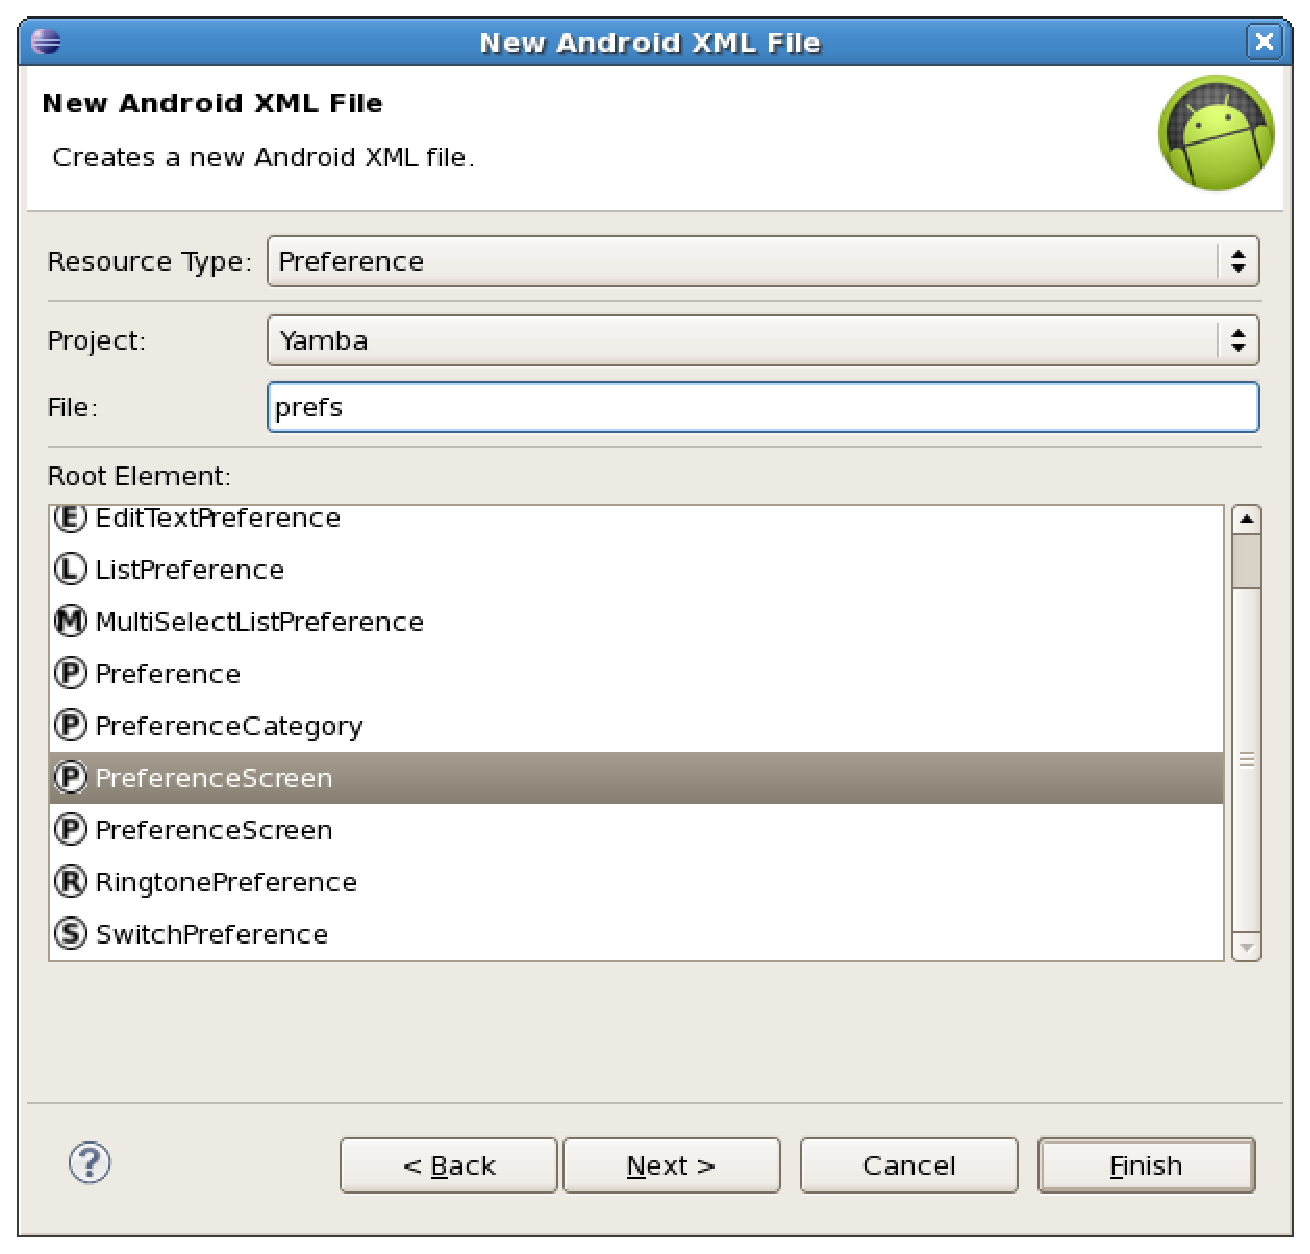
\includegraphics[width= 0.55 \textwidth]{newAndroidXMLFile.eps}
\end{frame}
%------------------------------------------------------------------------------
\begin{frame}
\frametitle{XML Elements}

	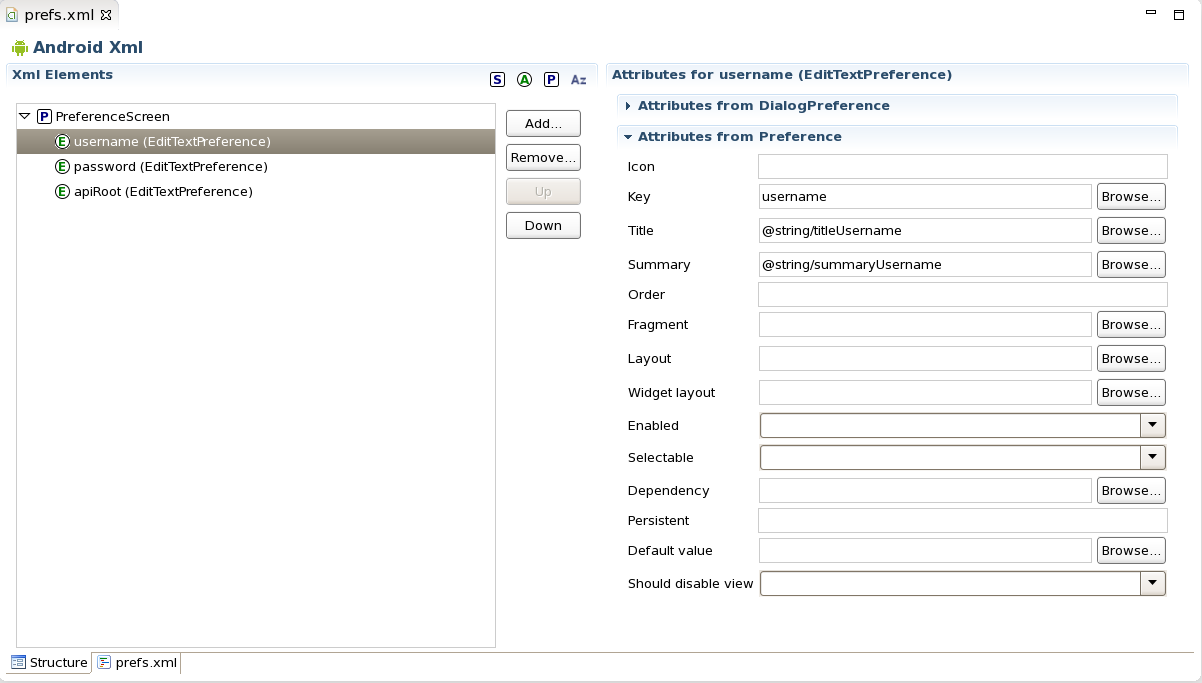
\includegraphics[width= 0.80 \textwidth]{xml-elements.eps}

\begin{description}
	\item[Key] A unique identifier for each preference item
	\item[Title] The preference name that the user will see
	\item[Summary] A short description of this preference item
\end{description}
	
\end{frame}
%------------------------------------------------------------------------------
\begin{frame}[containsverbatim]
\frametitle{\texttt{prefs.xml}}
\lstset{language=XML, style=eclipse}
\begin{adjustbox}{width=1.0 \textwidth}
\begin{lstlisting}[caption=res/xml/prefs.xml, basicstyle=\scriptsize,escapechar=$]
<?xml version="1.0" encoding="utf-8"?>
<PreferenceScreen xmlns:android="http://schemas.android.com/apk/res/android" >

    <EditTextPreference
        android:key="username"
        android:summary="@string/summaryUsername"
        android:title="@string/titleUsername" />
    <EditTextPreference
        android:key="password"
        android:summary="@string/summaryPassword"
        android:title="@string/titlePassword" />
    <EditTextPreference
        android:key="apiRoot"
        android:summary="@string/summaryApiRoot"
        android:title="@string/titleApiRoot" />

</PreferenceScreen>
\end{lstlisting}
\end{adjustbox}
\end{frame}
%------------------------------------------------------------------------------
\begin{frame}[containsverbatim]
\frametitle{\texttt{strings.xml}}
\lstset{language=XML, style=eclipse}
\begin{adjustbox}{width=1.0 \textwidth}
\begin{lstlisting}[caption=res/values/strings.xml, basicstyle=\scriptsize,escapechar=$]
<?xml version="1.0" encoding="utf-8"?>
<resources>

    <string name="app_name">Yamba1</string>
    <string name="action_settings">Settings</string>
    <string name="hello_world">Hello world!</string>
    <string name="titleStatus">Status Update</string>
    <string name="hintText">Please enter your 140 character status</string>
    <string name="buttonUpdate">Update</string>
    <string name="tittleUsername">Username</string> <!-- $\circled{1} $-->
    <string name="summaryUsername">Please enter your username</string>
    <string name="tittlePassword">Password</string>
    <string name="summaryPassword">Please enter your password</string>
    <string name="tittleApiRoot">API Root</string>
    <string name="summaryApiRoot">URL API for your service</string>

</resources>
\end{lstlisting}
\end{adjustbox}
\end{frame}
%------------------------------------------------------------------------------
\begin{frame}[containsverbatim]
\frametitle{\texttt{PrefsActivity.java}}
To create an activity, we create a new Java class. In Eclipse, select your package under
your src folder, right-click on the package, and select \texttt{New|Class}.
\lstset{language=java, style=eclipse}
\begin{adjustbox}{width=1.0 \textwidth}
\begin{lstlisting}[caption=src/com.artemisa.yamba/PrefsActivity.java, basicstyle=\scriptsize,escapechar=$]
// .
// .
// .
public class PrefsActivity extends PreferenceActivity { // $\circled{1}$
	@SuppressWarnings("deprecation")
	@Override
	protected void onCreate(Bundle savedInstanceState) { 
		// TODO Auto-generated method stub
		super.onCreate(savedInstanceState);

		$\sout{addPreferencesFromResource}$(R.xml.prefs); // $\circled{2}$
	}
}
\end{lstlisting}
\end{adjustbox}
\end{frame}
%------------------------------------------------------------------------------
\begin{frame}[containsverbatim]
\frametitle{Update the Manifest File}
We have a new \texttt{PrefsActivity} and must add it to the manifest file  \texttt{AndroidManifest.xml}
Choose the Application tab, and then under Application Nodes, choose \texttt{Add|Activity} and name it \texttt{PrefsActivity}

\centering
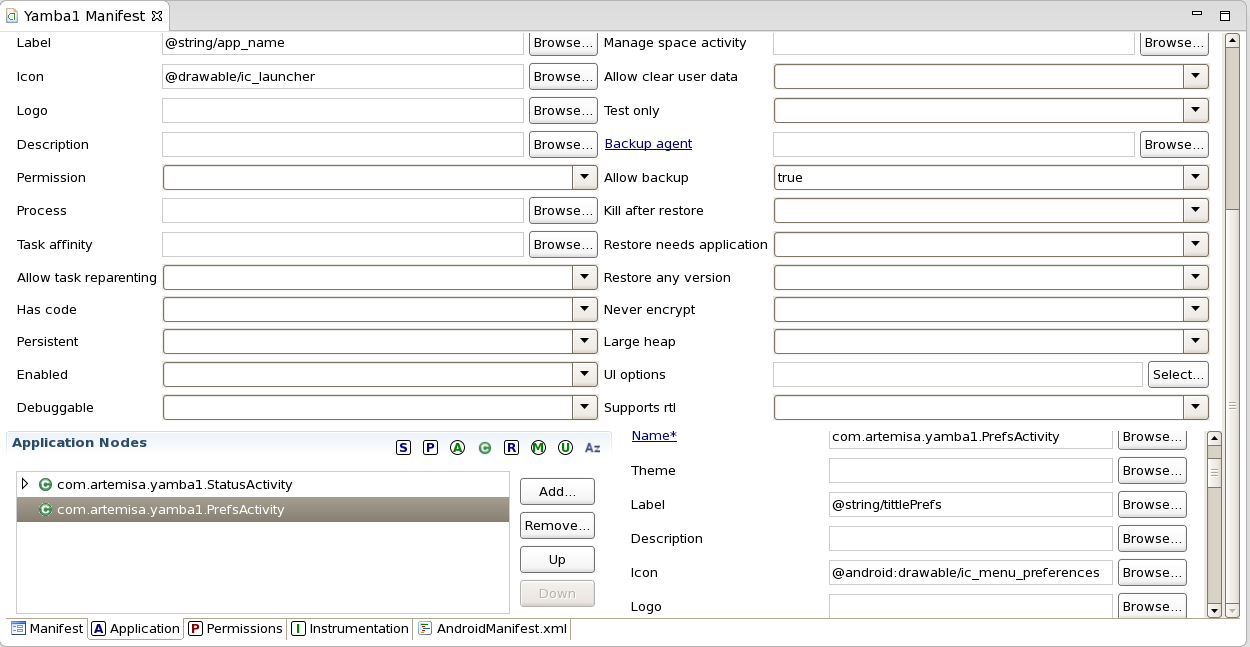
\includegraphics[width= 0.9 \textwidth]{yamba-manifiest.eps}

\end{frame}
%------------------------------------------------------------------------------
%------------------------------------------------------------------------------
\begin{frame}[containsverbatim]
\frametitle{Update the Manifest File}
\lstset{language=XML, style=eclipse}.
\begin{adjustbox}{width=1.0 \textwidth}
\begin{lstlisting}[caption=YambaManifiest.xml, basicstyle=\scriptsize,escapechar=$]
    <!-- . -->
    <!-- . -->
    <!-- . -->
        <activity
            android:name="com.artemisa.yamba1.StatusActivity"
            android:label="@string/app_name" >
            <intent-filter>
                <action android:name="android.intent.action.MAIN" />

                <category android:name="android.intent.category.LAUNCHER" />
            </intent-filter>
        </activity>

	<activity $\circled{1}$
            android:name="com.artemisa.yamba1.PrefsActivity"
            android:icon="@android:drawable/ic_menu_preferences"
            android:label="@string/tittlePrefs" >
        </activity>
    <!-- . -->
    <!-- . -->
    <!-- . -->
\end{lstlisting}
\end{adjustbox}
\end{frame}
%------------------------------------------------------------------------------
\subsection{The Options Menu}
\begin{frame}
\frametitle{The Options Menu}
The options menu is an Android user interface component that provides standardized
menus to applications. The menus appear at the bottom of the screen when the user
presses the Menu button on the device

To add support for the options menu to an application, we need to do the following:

\begin{enumerate}
\item Edit the \texttt{status.xml} resource where we specify what the menu consists of
\item Edit \texttt{onCreateOptionsMenu()} to the activity that should have this menu. This is
where we inflate the \texttt{status.xml} resource
\item Provide handling of menu events in \texttt{onOptionsItemSelected()}
\end{enumerate}
\end{frame}


%------------------------------------------------------------------------------
\begin{frame}
\frametitle{\texttt{status.xml}}

\centering
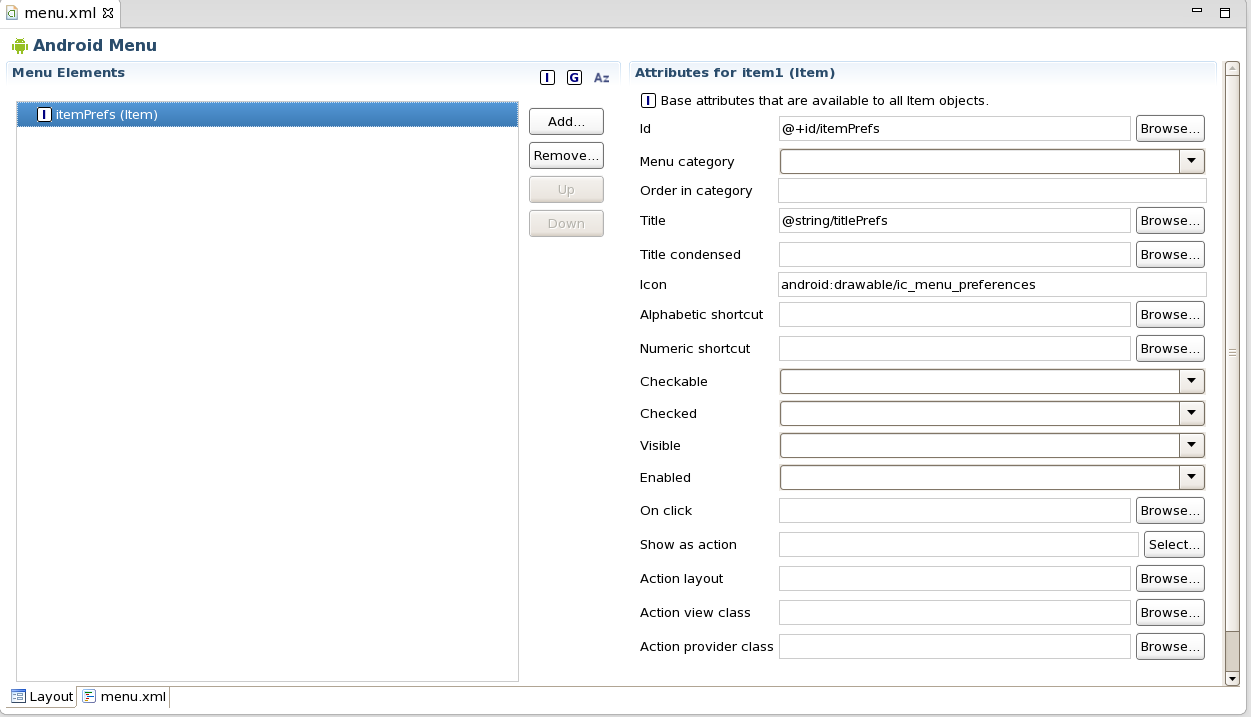
\includegraphics[width= 0.8 \textwidth]{menu.eps}
\end{frame}
%------------------------------------------------------------------------------
\begin{frame}[containsverbatim]
\frametitle{Update StatusActivity to Load the Menu}

The first time the Menu button is pressed, the system will call
the activity’s \texttt{onCreateOptionsMenu()} method to inflate the menu from the \texttt{status.xml}
resource

We need to update the \texttt{StatusActivity} to load up the options menu. To do that, edit
the \texttt{onCreateOptionsMenu()} method to \texttt{StatusActivity}

\lstset{language=java, style=eclipse}
\begin{adjustbox}{width=1.0 \textwidth}
\begin{lstlisting}[caption=src/com.artemisa.yamba/StatusActivity.java, basicstyle=\scriptsize,escapechar=$]
// Called first time user clicks on the menu button
@Override
public boolean onCreateOptionsMenu(Menu menu) { // $\circled{1}$
	MenuInflater inflater = getMenuInflater(); 
	inflater.inflate(R.menu.status, menu);
	return true; 
}
\end{lstlisting}
\end{adjustbox}


\end{frame}
%------------------------------------------------------------------------------
\begin{frame}[containsverbatim]
\frametitle{Update StatusActivity to Handle Menu Events}

We also need a way to handle various clicks on the menu items. To do that, we add
another callback method, \texttt{onOptionsItemSelected()}

\lstset{language=java, style=eclipse}
\begin{adjustbox}{width=0.90 \textwidth}
\begin{lstlisting}[caption=src/com.artemisa.yamba/StatusActivity.java, basicstyle=\scriptsize,escapechar=$]
// Called when an options item is clicked
@Override
public boolean onOptionsItemSelected(MenuItem item) {
	switch (item.getItemId()) { //
	case R.id.itemPrefs:
		$\colorbox{light-gray}{startActivity(new Intent(this, PrefsActivity.class));}$// $\circled{1}$
		break;
	}
	return true; //
}

\end{lstlisting}
\end{adjustbox}
\end{frame}
%------------------------------------------------------------------------------
\begin{frame}[containsverbatim]
\frametitle{Shared Preferences}
\begin{itemize}
\item Now that we have a preference activity and a way to save our username, password, and
API root, it is time to make use of it. To programmatically access your preferences, we'll
use the \texttt{SharedPreference} class provided by the Android framework.

\item This class is called \texttt{SharedPreference} because this preference is easily accessible from
any component of this application (activities, services, broadcast receivers, and content
providers)
\end{itemize}
\end{frame}
%------------------------------------------------------------------------------
\begin{frame}[allowframebreaks,containsverbatim]
\frametitle{The StatusActivity Java Class}
\lstset{language=java, style=eclipse, breaklines=true, tabsize=2}
%\begin{adjustbox}{width=1.0 \textwidth}
\centering
\begin{lstlisting}[caption=src/com.artemisa.yamba/StatusActivity.java, basicstyle=\tiny, escapechar=! ]
// .
// .
// .
public class StatusActivity extends Activity implements OnClickListener,
		TextWatcher, OnSharedPreferenceChangeListener { \\ !\circled{1}!

	// .
	// .
	// .
	private TextView textCount;

	private SharedPreferences prefs; !\circled{2}!

	@Override
	protected void onCreate(Bundle savedInstanceState) {
		// .
		// .
		// .
		editText.addTextChangedListener(this);

		// Setup preferences
		prefs = PreferenceManager.getDefaultSharedPreferences(this); // !\circled{3}!
		prefs.registerOnSharedPreferenceChangeListener(this);
	}

	// .
	// .
	// .

	private class PostToTwitter extends AsyncTask<String, Integer, String> {
		@Override
		protected String doInBackground(String... params) {
			// TODO Auto-generated method stub
			try {
				!\colorbox{light-gray}{Twitter.Status status = getTwitter().setStatus(params[0]);}! // !\circled{4}!
				return status.text;

			} catch (TwitterException e) {
				Log.e(TAG, e.toString());
				e.printStackTrace();
				return "Failed to post";
			}
		}

		// .
		// .
		// .
	}
	// .
	// .
	// .
	private Twitter getTwitter() { // !\circled{4}!
		if (twitter == null) { //
			String username, password, apiRoot;
			username = prefs.getString("username", ""); //
			password = prefs.getString("password", "");
			apiRoot = prefs.getString("apiRoot",
					"http://yamba.marakana.com/api");
			// Connect to twitter.com
			twitter = new Twitter(username, password); //
			twitter.setAPIRootUrl(apiRoot); //
		}
		return twitter;
	}

	@Override
	public void onSharedPreferenceChanged(SharedPreferences arg0, String arg1) { // !\circled{5}!
		// TODO Auto-generated method stub
		twitter = null;
	}

}

\end{lstlisting}
%\end{adjustbox}
\end{frame}
%------------------------------------------------------------------------------
\subsection{The Filesystem}
\begin{frame}[containsverbatim]
\frametitle{The Filesystem}
So, where does the device store these preferences? How secure is my username and
password? There are two ways for you to access the filesystem on an Android device: 

\begin{enumerate}
\item Via Eclipse \texttt{Window|Show View|Other\dots|Android|File Explorer}

\item  The command line \texttt{\$ adb shell}
\end{enumerate}

\end{frame}
%------------------------------------------------------------------------------
\begin{frame}[containsverbatim]
\frametitle{Filesystem Partitions}

\begin{itemize}
\item The system partition (\texttt{/system/}). Android operating system is located in the system partition
\item The SDCard partition (\texttt{/sdcard/})
\item The user data partition at (\texttt{/data/})
	\begin{itemize}
		\item \texttt{/data/app}
		\item \texttt{/data/data}
	\end{itemize}
\end{itemize}

\end{frame}
%------------------------------------------------------------------------------

\begin{frame}[containsverbatim]
\frametitle{Filesystem Security}
So, how secure is this? This is a common question posed by security folks. Storing
usernames and passwords in clear text always raises eyebrows
\begin{itemize}
\item Open up your commandline terminal and type
\end{itemize}

\centering{
\begin{adjustbox}{width=0.75 \textwidth}
\begin{lstlisting}[escapechar=!]
# !\textbf{cd}! /data/data/com.artemisa.yamba/shared_prefs
# !\textbf{cat}! com.artemisa.yamba_preferences.xml
<?xml version='1.0' encoding='utf-8' standalone='yes' ?>
<map>
<string name="password">password</string>
<string name="username">student</string>
<string name="apiRoot">http://yamba.marakana.com/api</string>
</map>
#
\end{lstlisting}
\end{adjustbox}}
\end{frame}
%------------------------------------------------------------------------------
\begin{frame}[fragile]
\frametitle{Git}
\begin{enumerate}
\item \texttt{git status}
\item \texttt{git add .}
\item \texttt{git status}
\item \texttt{git commit -a -m ``Preferences''}
\item \texttt{git remote add carmelocuenca https://github.com/carmelocuenca/Yamba.git}
\item \texttt{git push -u carmelocuenca master}
\end{enumerate}

\end{frame}
%------------------------------------------------------------------------------
\begin{frame}[containsverbatim]
\frametitle{Summary}
\centering
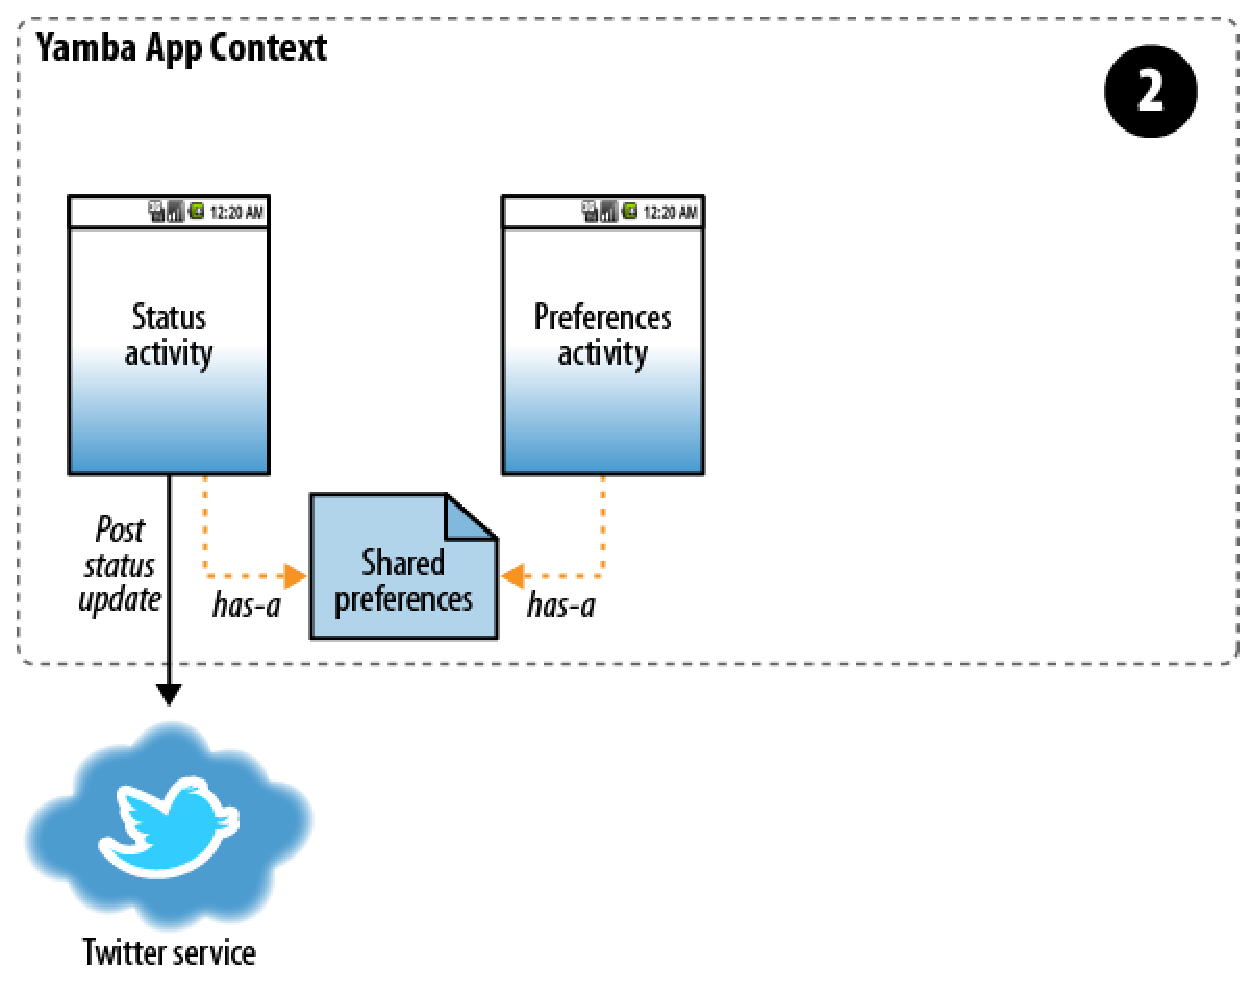
\includegraphics[width= 0.75 \textwidth]{fig-077.eps}
\end{frame}
%------------------------------------------------------------------------------



